\section{Least Squares}
The first three subsections of this section get inspiration from the book[]%~\cite{simon06}
, which explains the linear least squares topic in three gradual steps, to finally introduce the Kalman Filter in a natural and smooth way. The same approach is followed in this section, by first presenting the Linear Least Squares, thereafter the Weighted Linear Least Squares and then the Recursive approach. The fourth subsection is devoted to non-linear least squares topic.

The underlying idea and goal of the Least Squares topic is to \textit{find the system state that better explain your measurements}.

\subsection{Unweighted Linear Least Squares (UL-LS)}
Let be $\mathbf{x} \in \mathbb{R}^n$ the system state of~$n$ components, and~$\mathbf{z} \in \mathbb{R}^m$ a set of~$m$ measurements. Assuming the following linear model for the measurements:
\begin{equation}
 \mathbf{z} = \mathbf{H}\mathbf{x} + \mathbf{n}_z
\end{equation}
The goal of the Least Squares procedure is to estimate the state~$\mathbf{x}$ that better explain the measurements~$\mathbf{z}$. The problem in the above equation is that the true values of the noise~$\mathbf{n}_z$ for each measurement (each component) in~$\mathbf{z_i}$ are unknown. However, the noise is assumed to be a random variable following a normal distribution:
\begin{equation}
 \mathbf{n}_z \approx \mathcal{N}(0,\sigma^2_{n_z}\mathbf{I})
\end{equation}
so all the measurements are independent and have the same distribution, since the covariance matrix is an identity multiplied by a constant~$\sigma_{n_z}$.
We can define the \textit{expected measurement} vector as:
\begin{equation}
 \hat{\mathbf{z}} = \mathbf{H}\mathbf{x}
\end{equation}
which is the measurements we expect, according the model and given the state~$\mathbf{x}$. A measurement error can be also defined as: 
\begin{equation}
 \mathbf{e}_z = \mathbf{z} - \hat{\mathbf{z}}
\end{equation}
Given this error, the squared norm of it (squared length) seems to be an appropriate indicator to evaluate how big is this error, so it is defined the following function as the squared norm of the measurement error:
\begin{equation}
 f(\mathbf{e}_z) = \mathbf{e}^T_z\mathbf{e}_z = \sum^m_{i=1}e^2_i
\end{equation}
The criterion to find the state estimate,~$\hat{\mathbf{x}}$, that better explains the measurements is, therefore, to find those state~$\mathbf{x}$ that minimizes the function~$f(\mathbf{e}_z)$, so that minimizes the length of the error vector.
\begin{equation}
 \hat{\mathbf{x}} = \operatorname*{arg\,min}_{\mathbf{x}}\ f(\mathbf{e}_z)
\end{equation}
Developping the  expression of~$f(\mathbf{e}_z)$ to show explicitly its dependency on~$\mathbf{x}$:
\begin{equation}
 f(\mathbf{e}_z) = \mathbf{e}^T_z\mathbf{e}_z = (\mathbf{z}-\hat{\mathbf{z}})^T (\mathbf{z}-\hat{\mathbf{z}})
		 = (\mathbf{z}-\mathbf{H}\mathbf{x})^T(\mathbf{z}-\mathbf{H}\mathbf{x})
		 = \mathbf{z}^T\mathbf{z} - \mathbf{z}^T\mathbf{H}\mathbf{x} - \mathbf{x}^T\mathbf{H}^T\mathbf{z} + \mathbf{x}^T\mathbf{H}^T\mathbf{H}\mathbf{x}
\end{equation}
and then, forcing the derivative with respect to~$\mathbf{x}$ to be~$0$ to find the minimum:
\begin{equation}
  \frac{\partial f(\mathbf{e}_z)}{\partial \mathbf{x}} 
	= -\mathbf{z}^T\mathbf{H} -\mathbf{z}^T\mathbf{H} + 2\mathbf{x}^T\mathbf{H}^T\mathbf{H} = 0;
  \ \ \mathbf{x}^T\mathbf{H}^T\mathbf{H} = \mathbf{z}^T\mathbf{H};
  \ \ \mathbf{H}^T\mathbf{H}\mathbf{x} = \mathbf{H}^T\mathbf{z};
\end{equation}
and solving for~$\mathbf{x}$, we finally get the optimal state estimate as:
\begin{equation}
\label{eq:ul_least_squares}
 \hat{\mathbf{x}} = (\mathbf{H}^T\mathbf{H})^{-1}\mathbf{H}^T\mathbf{z}
\end{equation}
which provides an estimate of the state, given all the measurements~$\mathbf{z}$, a linear measurement model~$\mathbf{H}$, according to the criterion of minimal measurement error, and assuming all measurements have independent noise, but they follow the same normal distribution. 

\subsection{Weighted Linear Least Squares (WL-LS)}
In case we have a different confidence level for each measurement. Instead of throwing away the most uncertain measurements, it is wise to also use it, but \textit{weight} them less than the most certain ones. Moreover, some measurements can experience some level of covariance between them. The same linear measurement model than the one used in the unweighted case is assumed here:
\begin{equation}
 \mathbf{z} = \mathbf{H}\mathbf{x} + \mathbf{n}_z
\end{equation}
but in the weighted case, the measurement noise covariance can be a generic covariance matrix:
\begin{equation}
 \mathbf{n}_z \approx \mathcal{N}(0,\mathbf{C}_{n_z})
\end{equation}
The goal of the Weighted Least Squares procedure is to estimate the state~$\mathbf{x}$ that better explain the measurements~$\mathbf{z}$, taking into account different confidence levels for each of them.

To derive the final equation, a procedure similar to previous subsection is adopted, but in this case the function~$f(\mathbf{e}_z)$ to be minimized is the weighted norm, which can be interpreted as the Mahalanobis distance of the measurement error vector~$\mathbf{e}_z$ to the origin:
\begin{equation}
 f(\mathbf{e}_z) = \mathbf{e}^T_z\mathbf{C}^{-1}_{n_z}\mathbf{e}_z
\end{equation}
Imposing the same criterion of minimizing function~$f(\mathbf{e}_z)$ with respect to~$\mathbf{x}$, we get: 
\begin{equation}
 \frac{\partial f(\mathbf{e}_z)}{\partial \mathbf{x}} = 
 -\mathbf{z}^T\mathbf{C}^{-1}_{n_z}\mathbf{H} + \mathbf{x}^T\mathbf{H}^T\mathbf{C}^{-1}_{n_z}\mathbf{H} = 0; 
\end{equation}
and solving, the optimal state estimate is finally computed as:
\begin{equation}
\label{eq:wl_least_squares}
 \hat{\mathbf{x}} = (\mathbf{H}^T\mathbf{C}^{-1}_{n_z}\mathbf{H})^{-1}\mathbf{H}^T\mathbf{C}^{-1}_{n_z}\mathbf{z}
\end{equation}

\subsection{Recursive Weighted Linear Least Squares (RWL-LS)}
\label{subsec:recursive_ls}
The two previous subsections compute the state estimate~$\hat{\mathbf{x}}$ once all the measurements were available. This is usually called \textit{batch} mode, when you solve a problem off-line with all the measurements took into account in one single step. But real robotic estimation processes usually receive measurements one by one, since they usually come from some sensor source or detector process. Solving at each iteration the entire problem from the beginning would produce huge measurement vectors~$\mathbf{z}$ after a while, but even more critical, untreatable covariance matrices~$\mathbf{H}$ and~$\mathbf{C}_{n_z}$ to be inverted. So it is important to find a recursive approach to solve a linear least squares in such context. 

At a given iteration~$t$, we continue to assume a linear measurement model, which \textit{may} change at each iteration, as it is indicated with the~${}^t$ superindex: 
\begin{equation}
 \mathbf{z}^t = \mathbf{H}^t\mathbf{x}^t + \mathbf{n}^t_z,
\end{equation}
but now, a linear system model is also proposed which recursively updates the current state, based on the previous one: 
\begin{equation}
 \mathbf{x}^t = \mathbf{x}^{t-1} + \mathbf{K}^t(\mathbf{z}^t - \mathbf{H}^t\mathbf{x}^{t-1}).
\end{equation}
Given an initialization of~$\mathbf{x}^0$, right-sides of both equations above are known, exceptuating the matrix~$\mathbf{K}^t$, called the \textit{gain}, and the particular values of the mesurement noise in a given iteration,~$\mathbf{n}^t_z$. However the noise distribution is assumed to be known, as we did in the non-recursive case. In order to derive the final set of equations for the recursive algorithm, the goal is to find this gain matrix~$\mathbf{K}^t$. In that case, the criterion will change, and it will be to minimize the sum of the variances of the estimation error at iteration~$t$. So the function to minimize is:
\begin{equation}
 f(\mathbf{e}^t_x) = Tr\{\mathbf{C}^t_{x}\},
\end{equation}
where the operator $Tr\{\}$ is the trace of the matrix, which is the sum of all diagonal elements (variances) of the covariance matrix. Expressing the estimation error as: 
\begin{equation}
 \mathbf{e}^t_x = \mathbf{x}^t - \hat{\mathbf{x}}^t
\end{equation}
so the covariance matrix, by definition is the expectation of $\mathbf{e}_x\mathbf{e}^T_x$:
\begin{equation}
 \mathbf{C}^t_{x} = \mathcal{E}\{\mathbf{e}^t_x(\mathbf{e}^t_x)^T\}
\end{equation}
which after some maths (see[]%~\cite{simon06})
, leads to: 
\begin{equation}
 \mathbf{C}^t_{x} = (\mathbf{I}-\mathbf{K}^t\mathbf{H}^t)\mathbf{C}^{t-1}_x(\mathbf{I}-\mathbf{K}^t\mathbf{H}^t)^T
		    + \mathbf{K}^t\mathbf{C}^t_{n_z}(\mathbf{K}^t)^T
\end{equation}
Coming back to our minimization goal, 
\begin{equation}
 f(\mathbf{e}^t_x) = Tr\{\mathbf{C}^t_{x}\} \rightarrow \frac{\partial f(\mathbf{e}^t_x)}{\partial \mathbf{K}^t} = 0
\end{equation}
which finishes with the expression for the gain:
\begin{equation}
 \mathbf{K}^t = \mathbf{C}^{t-1}_x(\mathbf{H}^t)^T(\mathbf{H}^t\mathbf{C}^{t-1}_x(\mathbf{H}^t)^T+\mathbf{C}^t_{n_z})^{-1}
\end{equation}

The algorithm~\ref{alg:recursive_ls} summarizes all the steps for the recursive least squares approach. The algorithm requires three inputs to start looping: the initial guess for the state estimate,~$\mathbf{x}^0$, the initial guess for the covariance of the state estimate,~$\mathbf{C}^0_x$, and the measurement model,~$\mathbf{H}^t$ which may, or may not, be time dependent. The algorithm provides at the end of each iteration~$t$ the state estimate that better explain the measurements received up to~$t$, according the criterion of minimizing the trace of~$\mathbf{C}^t_x$.
\begin{algorithm}
\caption{Recursive Weighted Linear Least Squares}
INPUTS: $\hat{\mathbf{x}}^0,\mathbf{C}^0_x,\mathbf{H}^t,\mathbf{C}^t_{n_z}$\\
OUTPUT: $\hat{\mathbf{x}}^t,\mathbf{C}^t_x$, at each iteration
\begin{algorithmic}
\STATE INIT: $\hat{\mathbf{x}}^0,\mathbf{C}^0_x$
\STATE FOR EACH ITERATION
\STATE \hspace{1cm} $\mathbf{H}^t$ //Compute it, if it is not constant
\STATE \hspace{1cm} $\hat{\mathbf{z}}^t = \mathbf{H}^t\hat{\mathbf{x}}^{t-1}$ //Compute the expected measurement 
\STATE \hspace{1cm} $\mathbf{K}^t = \mathbf{C}^{t-1}_x(\mathbf{H}^t)^T(\mathbf{H}^t\mathbf{C}^{t-1}_x(\mathbf{H}^t)^T+\mathbf{C}^t_{n_z})^{-1}$ 
//Compute the gain
\STATE \hspace{1cm} $\hat{\mathbf{x}}^t = \hat{\mathbf{x}}^{t-1} + \mathbf{K}^t(\mathbf{z}^t - \hat{\mathbf{z}}^t)$ //Update the state estimate
\STATE \hspace{1cm} $\mathbf{C}^t_{x} = (\mathbf{I}-\mathbf{K}^t\mathbf{H}^t)\mathbf{C}^{t-1}_x(\mathbf{I}-\mathbf{K}^t\mathbf{H}^t)^T
		    + \mathbf{K}^t\mathbf{C}^t_{n_z}(\mathbf{K}^t)^T$ //Update the covariance of the state estimate
\RETURN $\hat{\mathbf{x}}^t,\mathbf{C}^t_x$		    
\STATE END FOR
\end{algorithmic}
\label{alg:recursive_ls}
\end{algorithm}

\paragraph{Example \theexamplecounter. Estimate a constant velocity from wheel encoders.}
\stepcounter{examplecounter}
This example assumes a 4-wheeled vehicle running at constant forward velocity~$v$ and rotational rate~$\omega$ on a plane.
We want to estimate these two variables, from the measurements we get from each wheel encoder. So, the main step we have to solve is to find the measurement model, which relates the state~$\mathbf{x}=[v\ \omega]$ with these measurements.
\begin{figure}[h!]
  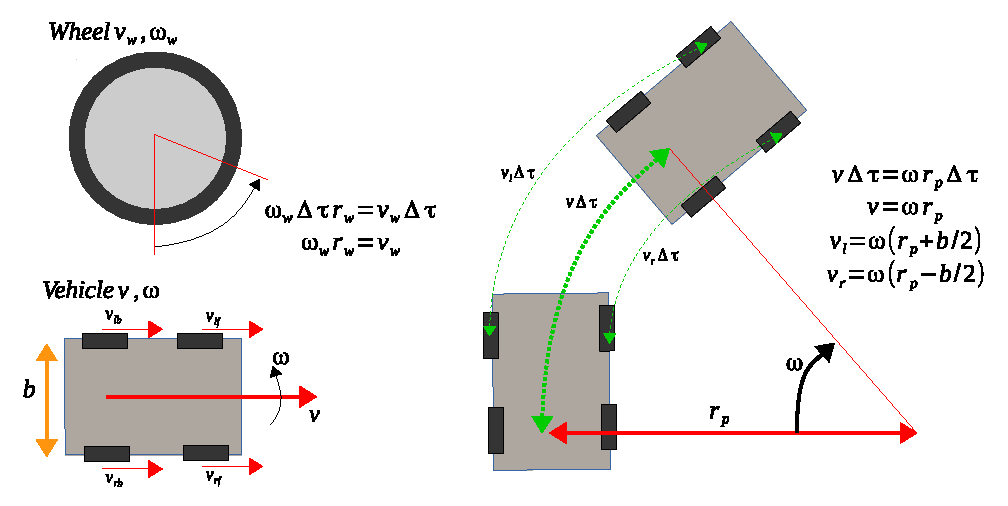
\includegraphics[width=1\linewidth]{figures/wheel-4diff_kinematics.eps}
  \caption{Differential 4-wheel kinematics: from wheel rotational rates to vehicle linear and rotational velocities~$v,\omega$.}
  \label{fig:wheel-4diff_kinematics}
\end{figure}

The measurements we have are the four linear velocities provided by the four encoders mounted at each wheel axis (see figure~\ref{fig:wheel-4diff_kinematics}). These linear velocities are directly the rotational velocities,~$\omega_w$ reported by each encoder multiplied by the wheel radius,~$r_w$:
\begin{equation}
v_{lf} = \omega_{lf}r_{lf};\ v_{lb} = \omega_{lb}r_{lb};\ v_{rf} = \omega_{rf}r_{rf};\ v_{rb} = \omega_{rb}r_{rb}
\end{equation}
where $\omega_{**}$, $v_{**}$ and~$r_{**}$ are rotational and linear speeds and radius for each wheel (left/right front/back). We consider the radius of the wheels to be precisely known,~$r_w$, so the only random variable is each rotational speed measurement, which leads to random variables at linear speed for each wheel. 

From the kinematics of a 4-wheeled platform (Figure~\ref{fig:wheel-4diff_kinematics}), we have the following two equations, for left and right velocities, according to the rotational rate of the vehicle. These equations relate the arc run by the robot, for the left-wheels and for the right ones, during a $\Delta\tau$ time step:
\begin{equation}
\begin{array}{cc}
 v_l\Delta\tau = & \omega\Delta\tau(r_c+\frac{b}{2}) \\
 v_r\Delta\tau = & \omega\Delta\tau(r_c-\frac{b}{2}) 
\end{array}
\label{eq:v_l_v_r}
\end{equation}
where the curvature radius of the vehicle's trajectory,~$r_c$, is provided by the relation~$v=\omega r_c$. Rearranging terms, we finish with the following two equations which explain measurements~$v_{l*},v_{r*}$ as a function of the system state~$\mathbf{x}=[v\ \omega]^T$
\begin{equation}
\begin{array}{cc}
 v_{l*} = v+\omega\frac{b}{2} \\
 v_{r*} = v-\omega\frac{b}{2}
\end{array}
\end{equation}
so the measurement process is modelled as:
\begin{equation}
 \mathbf{z}^t = \mathbf{H}^t\mathbf{x}^t + \mathbf{n}^t_z 
\end{equation}
where each term of the above equation is:
\begin{equation}
 \mathbf{z}^t =
 \left[
 \begin{array}{c}
  v_{lf}\\
  v_{lb}\\
  v_{rf}\\
  v_{rb}
 \end{array}
 \right]; \ 
 \mathbf{H}^t = \mathbf{H} = 
 \left[
 \begin{array}{cc}
  1 & b/2 \\
  1 & b/2 \\
  1 & -b/2 \\
  1 & -b/2 \\
 \end{array}
 \right];\ 
 \mathbf{x}^t=
 \left[
 \begin{array}{c}
  v\\
  \omega
 \end{array}
 \right]^t;\ 
 \mathbf{n}^t_z \sim \mathcal{N}(\mathbf{0},\mathbf{C}_{n_z})
\end{equation}
At this point, we need to model the measurement noise, by setting the coefficients of the~$\mathbf{C}_{n_z}$ matrix according of data and knowledge we may have coming from the device datasheets and/or the measurement procedures (misscalibrations, missynchronizations, noise, unmodelled vehicle slippages, ... ). To illustrate better the effect of different uncertainty levels on measurement, the example propose to consider that the front encoders are cheaper than the back ones. With all this in mind, we consider~$\sigma_{.f}=5cm/s^2$ and~$\sigma_{.b}=1cm/s$, and we set covariance terms to $0.5^2 cm^2/s$, so the final measurement covariance matrix is (constant in time):
\begin{equation}
 \mathbf{C}_{n_z} = 
 \left[
 \begin{array}{cccc}
  0.05^2 & 0.005^2 & 0.005^2 & 0.005^2 \\
  0.005^2& 0.01^2  & 0.005^2 & 0.005^2 \\
  0.005^2& 0.005^2 & 0.05^2  & 0.005^2 \\
  0.005^2& 0.005^2 & 0.005^2 & 0.01^2
 \end{array}
 \right]
\end{equation}

Finally, we need the initial guess for the state estimate and state covariance. The initial guess for the state can be set by some knowledge about the system, or may be by collecting a short initial subset of measurements, computing the mean of them and solving the expression:
\begin{equation}
\begin{array}{cc}
 v = \frac{v_r+v_l}{2} \\
 \omega = \frac{v_l-v_r}{b}
\end{array}
\end{equation}
which comes from adding and substracting the two equations in~\ref{eq:v_l_v_r}. Fo state covariance matrix, the initial guess have to be enough \textit{noisy} to allow the algorithm to take effect from measurements appropiately, so it could be set to: 
\begin{equation}
 \mathbf{C}^0_{x} = 
 \left[
 \begin{array}{cc}
  1^2 & 0 \\
  0 & 0.2
  \end{array}
 \right]
\end{equation}
which indicates $\sqrt{1}m/s$ in linear standard deviation and $\sqrt{0.2}rad/s$ in rotational rate standard deviation. 

If we don't have actual measurements from a set of encoders, to simulate the measurement set is required to generate them syntethically, taking into account some stathistics. This is performed at the first lines of the SciLab code below.  The code continues initiliazing the involved matrixes, and then it goes to the main loop that solves iteratively the least squares estimate for~$v$ and~$\omega$.
\begin{mdframed}
\tiny
\begin{verbatim} 
//clear
clear;

//user entries 
n_iter = 200; //number of iterations
bb = 2; //vehicle axis width
v_true = 2.17; //true linear vehicle speed[m/s]
w_true = 0.12; //true rotational vehicle speed [rad/s]

//above vehicle linear and rot speeds, causes true left and right wheel linear speeds
v_l_true = v_true + w_true*bb/2;
v_r_true = v_true - w_true*bb/2;

//Generate noisy measurements, for each of the four encoders, at each iteration
//Measurements are each wheel linear velocity, arranged as: z=[v_lf;v_lb;v_rf;v_rb] (l:left, r:right, f:front, b:back)
sigma_v_f = 0.05; //std dev of linear wheel speed, for front encoders [m/s]. They are cheaper than back ones!
sigma_v_b = 0.01; //std dev of linear wheel speed, for back encoders [m/s]. They are better than front ones!
rand("normal");//set the distribution type to the generator
v_lf = v_l_true + rand(1,n_iter)*sigma_v_f;//left front measurements
v_lb = v_l_true + rand(1,n_iter)*sigma_v_b;//left back measurements
v_rf = v_r_true + rand(1,n_iter)*sigma_v_f;//right front measurements
v_rb = v_r_true + rand(1,n_iter)*sigma_v_b;//right back measurements
z = [v_lf;v_lb;v_rf;v_rb]; //stack all measurements in a single matrix

//****************** Recursive Least Squares starts here. ************************
//initial guess (state mean and covariance)
x_est = [0;0]; //for the state: [v w]
C_x = [1 0; 0 0.2]; //for the state covariance

//measurement model (constant)
H = [1 bb/2; 1 bb/2; 1 -bb/2; 1 -bb/2;]

//sets measurement process covariance (use values of sigma previously used to generate data)
sigma2_v_fb = 0.005^2; //covariance front-back linear wheel speeds [m^2/s^2]
C_nz = [sigma_v_f^2 sigma2_v_fb sigma2_v_fb sigma2_v_fb; sigma2_v_fb sigma_v_b^2 sigma2_v_fb sigma2_v_fb;
          sigma2_v_fb sigma2_v_fb sigma_v_f^2 sigma2_v_fb; sigma2_v_fb sigma2_v_fb sigma2_v_fb sigma_v_b^2];
          
//init other usefuls matrixes
I = eye(2,2); //set a 2x2 Identity
x_est_array = []; //state estimate at each iteration
tr_C_x_array = []; //trace of state covariance matrix

//recursive loop
for ii=1:n_iter
    //compute recursive weighted linear least squares
    z_exp = H*x_est; //expected measurememt
    K = C_x*H'*inv(H*C_x*H'+C_nz); //gain
    x_est = x_est + K*(z(:,ii)-z_exp); //update state estimate
    C_x = (I-K*H)*C_x*(I-K*H)' + K*C_nz*K'; //update state covariance
    
    //collect results
    x_est_array = [x_est_array x_est]; 
    tr_C_x_array = [tr_C_x_array trace(C_x)];
end
//****************** Recursive Least Squares ends here. ************************

//plots
figure('BackgroundColor',[1 1 1]);
plot(x_est_array(1,:));
ph = gca(); // handle
ph.x_label.text = 'iteration';
ph.y_label.text = 'Linear Velocity, v[m/s]';
ph.axes_visible = ["on","on","off"]
ph.grid = [1,1];
ph.auto_scale="on";
figure('BackgroundColor',[1 1 1]);
plot(x_est_array(2,:));
ph = gca(); // handle
ph.x_label.text = 'iteration';
ph.y_label.text = 'Rotational Velocity, w[rad/s]';
ph.axes_visible = ["on","on","off"]
ph.grid = [1,1];
ph.auto_scale="on";
figure('BackgroundColor',[1 1 1]);
plot(tr_C_x_array);
ph = gca(); // handle
ph.x_label.text = 'iteration';
ph.y_label.text = 'Trace(C_x)';
ph.axes_visible = ["on","on","off"]
ph.grid = [1,1];
ph.auto_scale="on";
\end{verbatim} 
\end{mdframed}

Figure~\ref{fig:vw_plot_rw-ls} shows the evolution of each component of the state estimate~$\hat{\mathbf{x}}=[\hat{v}\ \hat{\omega}]$, while the recursive algorithm iterates, as well as how the trace of the covariance matrix~$\mathbf{C}^t_x$ drops, indicating that the output state estimate decreases its uncertainty. 
\begin{figure}[h!]
  \centering
  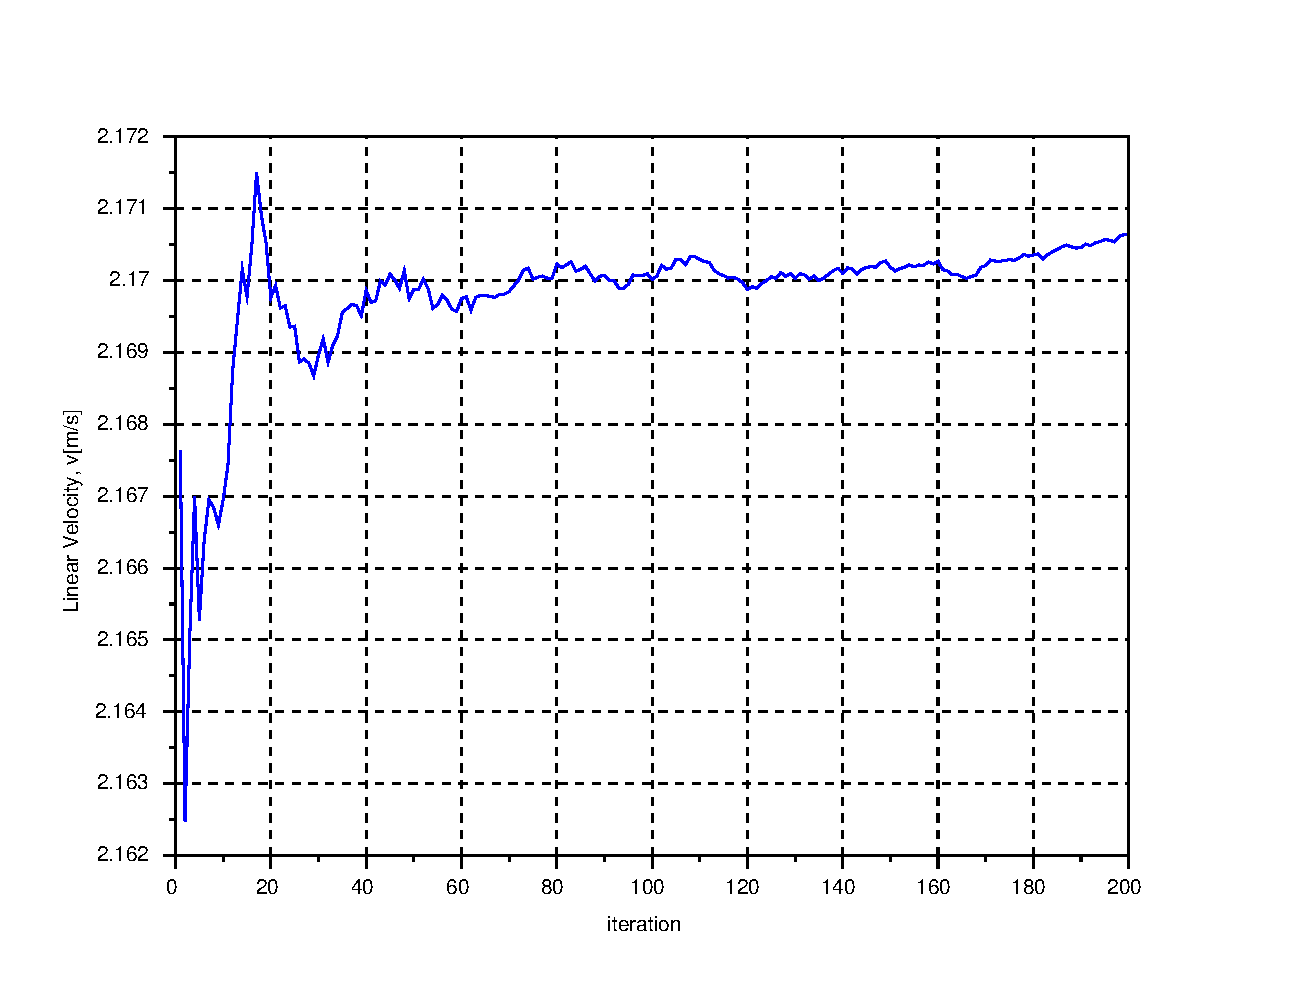
\includegraphics[width=0.32\linewidth]{figures/v_linear_rw-ls.eps}
  \hspace{0mm}
  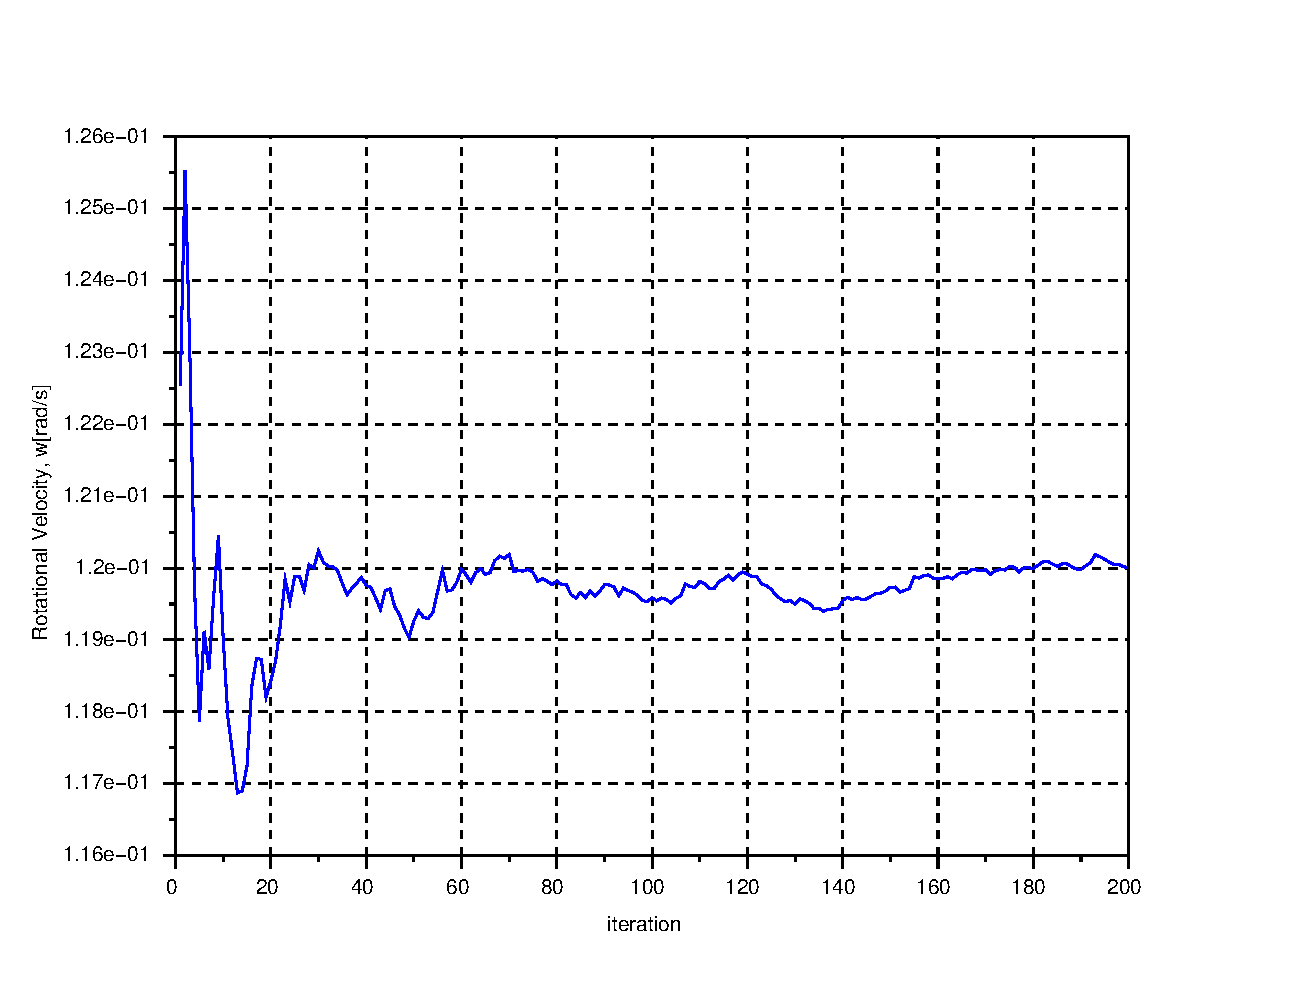
\includegraphics[width=0.32\linewidth]{figures/w_rotational_rw-ls.eps}
  \hspace{0mm}
  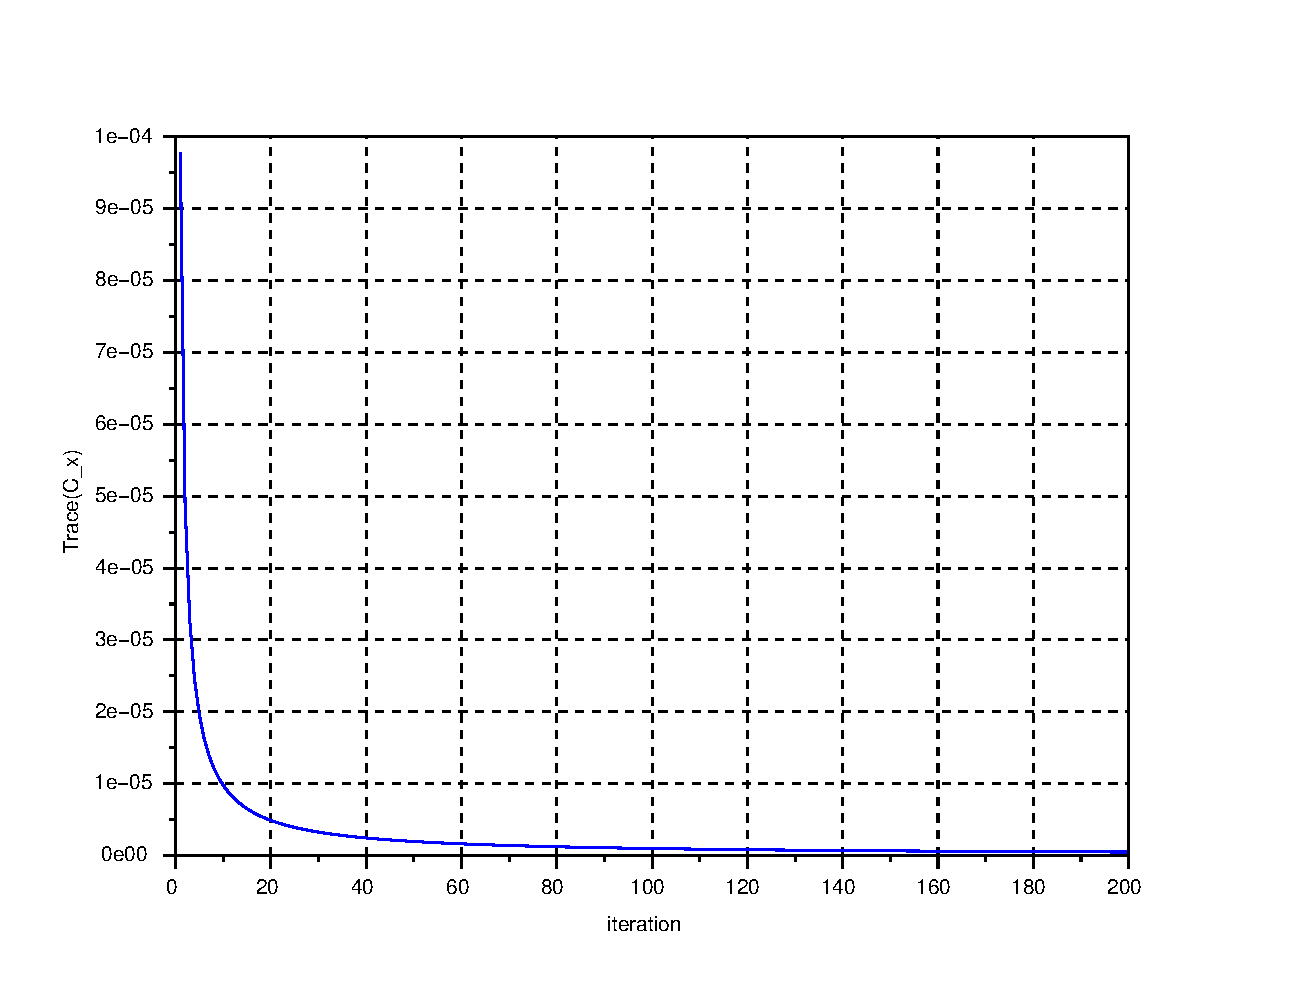
\includegraphics[width=0.32\linewidth]{figures/trCx_rw-ls.eps}
  \hspace{0mm}
  \caption{Evolution of linear (left) and rotational (center) speeds, and trace of covariance matrix (right), while the algorithm iterates.}
  \label{fig:vw_plot_rw-ls}
\end{figure}



\subsection{Linear Least Squares on homeogeneous systems (LS-HS)}
\label{subsec:ls_homogeneous}
Sometimes the problem to solve has different starting situation: 
\begin{equation}
 \mathbf{A}\mathbf{x} = \mathbf{0}
\end{equation}
where $\mathbf{x}$ is the state vector (unknown parameters) and the matrix $\mathbf{A}$ contains the measurement data. A typical case is when estimating the parameters of an homogeneous line or plane, given a set of data points. Beyond the trivial solution, which is the null vector, the least squares solution of such systems of equations is computed through the SVD decomposition of matrix $\mathbf{A}$:
\begin{equation}
 \mathbf{A} = \mathbf{UDV}^T
\end{equation}
And the result for~$\mathbf{x}$ is in the last column of matrix~$\mathbf{V}$. More details on SVD can be found at subsection~\ref{subsec:matrix_svd}) of this document.










\subsection{Non-Linear Least Squares (NL-LS)}


